% title: A tool-use agent updates its loop state
% description: The bounded loop calls the model while state.active is true. Search updates history and keeps the state active. Done sets the result and makes the state inactive. Termination returns state.result.
\documentclass[tikz,border=5pt]{standalone}
\usetikzlibrary{arrows.meta,calc,shapes.geometric}
\definecolor{numeric}{HTML}{4477AA}
\definecolor{textual}{HTML}{AA4499}

\tikzset{
    box/.style={draw, line width=0.8pt, minimum height=0.8cm,
                minimum width=1.8cm, inner sep=6pt, align=center},
    ir/.style={box},
    flow/.style={-{Stealth[length=5pt]}, line width=0.9pt},
    feedback/.style={flow, dashed},
    note/.style={font=\small, align=center},
    choice/.style={diamond, draw, line width=0.8pt,
                   aspect=2, inner sep=2pt, align=center},
}

\newcommand{\irframe}[2]{
    \draw[line width=0.8pt] #1 rectangle #2;
}

\newcommand{\transformarrow}[4][above]{
    \draw[flow] (#2) -- node[#1=6pt,note] {#4} (#3);
}

\begin{document}
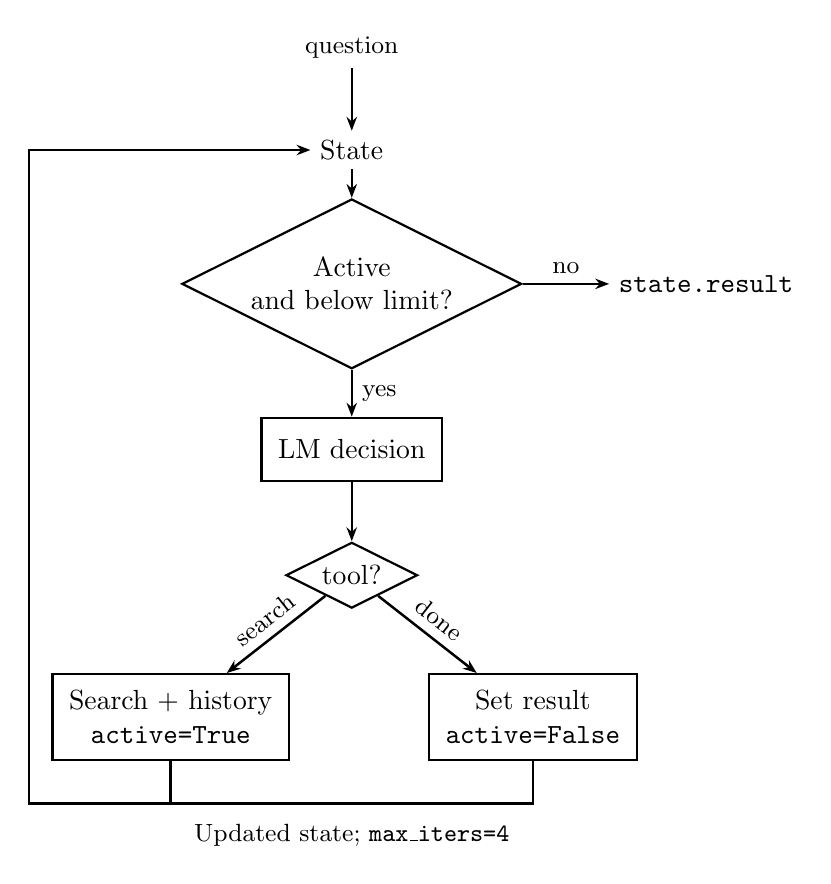
\begin{tikzpicture}

    \node[note] (question) at (0,3.3) {question};
    \node[align=center] (state) at (0,2) {State};
    \node[choice] (condition) at (0,0.3) {Active\\and below limit?};
    \node[box] (model) at (0,-1.8) {LM decision};
    \node[choice] (tool) at (0,-3.4) {tool?};
    \node[box] (search) at (-2.3,-5.2) {Search + history\\\texttt{active=True}};
    \node[box] (done) at (2.3,-5.2) {Set result\\\texttt{active=False}};
    \node (result) at (4.5,0.3) {\texttt{state.result}};
    \draw[flow] (question) -- (state);
    \draw[flow] (state) -- (condition);
    \draw[flow] (condition) -- node[right,note] {yes} (model);
    \draw[flow] (condition) -- node[above,note] {no} (result);
    \draw[flow] (model) -- (tool);
    \draw[flow] (tool) -- node[above,sloped,note] {search} (search);
    \draw[flow] (tool) -- node[above,sloped,note] {done} (done);
    \coordinate (updated) at (0,-6.3);
    \draw[line width=0.9pt] (search.south) |- (updated);
    \draw[line width=0.9pt] (done.south) |- (updated);
    \draw[flow] (updated) -- (-4.1,-6.3) -- (-4.1,2) -- (state.west);
    \node[note] at (0,-6.7) {Updated state; \texttt{max\_iters=4}};

\end{tikzpicture}
\end{document}
